\Chapter{Megvalósítás}


\section{Adatbázisok és modellek}
A programban a drón, és telemetria adatmodell a legfontosabb.
Ezeket az adatokat olvassuk és mentjük,illetve szükségesek az azonosításhoz vagy bármilyen értelmes következtetéshez a problémához kapcsolódóan.

\subsection{Modellek az adatközpont programban}
\subsubsection{Telemetria modell}
A programban a telemetria modell a következőképpen néz ki:
\begin{python}
    package models

    import "time"

    type Telemetry struct {
        Speed              float64          `json:"speed" db:"speed"`
        Location           GPS              `json:"location" `
        Altitude           float64          `json:"altitude" ` // in meters
        Bearing            float64          `json:"bearing" `
        Acceleration       float64          `json:"acceleration" `
        BatteryLevel       int              `json:"battery_level" `
        BatteryTemperature int              `json:"battery_temperature" `
        MotorTemperatures  []int            `json:"motor_temperatures" `
        Errors             []TelemetryError `json:"errors" db:"errors" `
        TimeStamp          time.Time        `json:"time_stamp" `
        DroneID            int              `json:"drone_id" `
    }

    type TelemetryError int

    const (
        MotorFailure TelemetryError = iota
        BeaconSignalStrengthLow
        BeaconSignalInterference
        BeaconTemperatureTooHigh
        GPSInt	eference
        GPSSignalLost
        GPSTemperatureTooHigh
        ProcessorTemperatureTooHigh
        BatteryFailure
        FailedToEjectPackage
        PackageLost
        DestinationDistanceTooFar
    )

    type GPS struct {
        Latitude  float64 `json:"latitude" bson:"latitude"`
        Longitude float64 `json:"longitude" bson:"longitude"`
    }

\end{python}


\subsubsection{Drone modell}
\begin{python}
    type Drone struct {
        ID           int           `json:"id" db:"drone_id" bson:"id"`
        Telemetry    Telemetry     `json:"telemetry" bson:"telemetry"`
        Parcel       Parcel        `json:"parcel"`
        Destinations []Destination `json:"destinations"`
        Consumption  float64       `json:"consumption"`
        Weight       float64       `json:"weight"`
        State        DroneState    `db:"state" bson:"state"`
    }

    type DroneState string

    const (
    DroneFree     DroneState = "free"
    DroneInFlight DroneState = "in-flight"
    )
\end{python}


\subsubsection{Parcel modell (szállítandó csomag)}
A drónok által szállított csomag így néz ki:
\begin{python}
    type Parcel struct {
        ID            int             `json:"id" db:"id" bson:"id"`
        TrackingID    string          `json:"tracking_id" `
        Name          string          `json:"name" db:"name" bson:"name"`
        Weight        float64         `json:"weight" db:"weight"`
        Location      GPS             `json:"location" bson:"location"`
        FromAddress   ShippingAddress `json:"from_address"`
        ToAddress     ShippingAddress `json:"to_address"`
        DropOffSite   GPS             `bson:"drop_off_site" `
        AssignedDrone int             `json:"assigned_drone" `
    }
\end{python}

\subsection{Relációs adatbázis, PostgreSQL modell}
A relációs adatbázissal is működik a szimuláció.
\paragraph{Relációs modell \ref{fig:postgres} } \mbox{} \\

\begin{figure}[h]
    \centering
    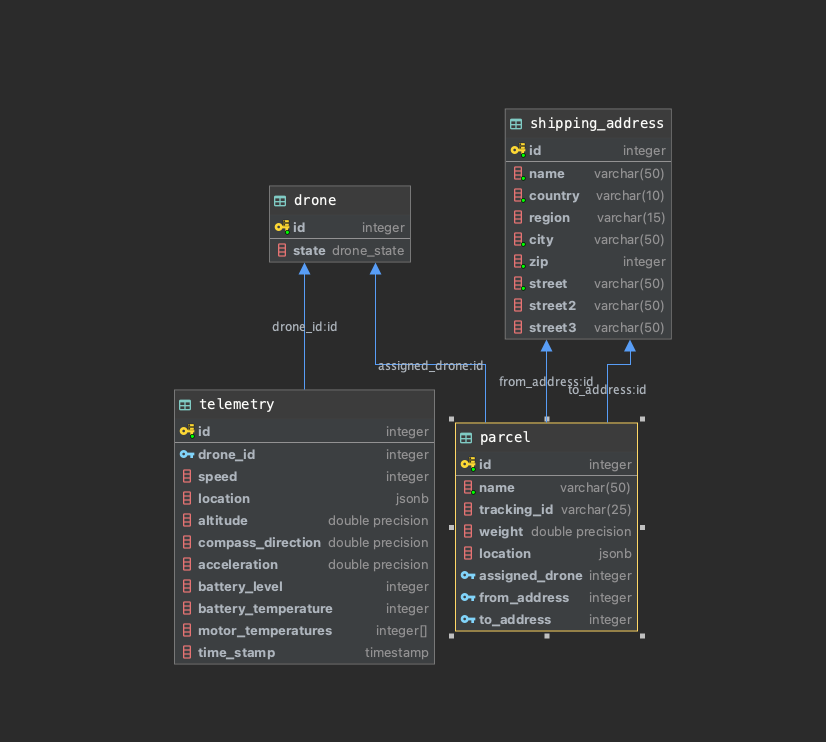
\includegraphics[scale=0.4]{images/postgres.png}
    \caption{PostgreSQL adatbázis modell}
    \label{fig:postgres}
\end{figure}

%TODO: ide táblázattal megcsinalni a relacios modellt


\paragraph{Lost Update probléma} \mbox{} \\
A legtöbb relációs adatbázis támogatja a tranzakciókat. A tranzakciók ACID tulajdonságokkal bírnak.
Adatbázisok esetén az ACID az Atomicity (atomiság), Consistency (konzisztencia), Isolation (izoláció), és Durability (tartósság) rövidítése. Ezek nélkül az adatbázis integritása nem garantálható.
A PostgreSQL többféle izolációs szintet biztosít a tranzakciókhoz \cite{postgres-transaction}. A Lost Update problémát garantáltan megoldja a PostgreSQL `Serializable` izolációs szintje.
\begin{table}[h]
    \centering
    \caption{ Standard SQL Transaction Isolation Levels}
    \begin{tabular}{l|c|c|c|}
Isolation Level & Dirty Read  & Nonrepeatable Read & Phantom Read\\
        \hline
Read uncommitted  & Possible & Possible & Possible \\
\hline
Read committed & Not possible & Possible & Possible \\
\hline
Repeatable read & Not possible & Not possible & Possible \\
\hline
Serializable & Not possible & Not possible & Not Possible \\
        \hline
    \end{tabular}
\end{table}

\subsection{Dokumentum alapú adatbázis, MongoDB}

A telepítéshez
\begin{python}
    use drone_delivery
\end{python}

\begin{python}

    db.createUser(
        {
        user: "drone-user",
        pwd: "drone-pwd",
        roles: [
            {
            role: "readWrite",
            db: "drone_delivery"
        }
        ]
    }
    )
\end{python}



\section{A programok felépítése a követelmények alapján}
%TODO: ide irni Hexagonalrol, es az implementaciorol


\section{Szállítási probléma a programban}
\subsubsection{Az adatközpont távolság számítása}
Az adatközpont program az Ortodroma számítást használja, hogy kiszámolj a távolságot a legoptimálisabb útvonal keresése közben.
Ez a számítás nem tökéletes, nem ér fel egy nagyon pontos GPS rendszerrel de a problémát tökéletesen megoldja.
\begin{python}
    func (s *service) CalculateDistance(lat1, lng1, lat2,
            lng2 float64, unit ...string) float64 {
        const PI = float64(math.Pi) //3.141592653589793

        radlat1 := PI * lat1 / 180
        radlat2 := PI * lat2 / 180

        theta := lng1 - lng2
        radtheta := PI * theta / 180

        dist := math.Sin(radlat1)*math.Sin(radlat2) +
        math.Cos(radlat1)*math.Cos(radlat2)*math.Cos(radtheta)

        if dist > 1 {
            dist = 1
        }

        dist = math.Acos(dist)
        dist = dist * 180 / PI
        dist = dist * 60 * 1.1515

        if len(unit) > 0 {
            if unit[0] == "K" {
                dist = dist * 1.609344
            } else if unit[0] == "N" {
                dist = dist * 0.8684
            } else if unit[0] == "METER" {
                dist = dist * 1.609344 * 1000
            }
        }

        return dist
    }
\end{python}
\subsubsection{A drón-raj program számításai}
A pontos szimulációs értékekhez egy sokkal komolyabb könyvtárat használunk, ami megfelel a WGS84 GPS rendszernek.
Ezzel a könyvtárral pontos adatokat tudunk generálni a drón helyzetéről, irányáról.


\begin{python}

    geo := ellipsoid.Init("WGS84", ellipsoid.Degrees, ellipsoid.Meter,
    ellipsoid.LongitudeIsSymmetric, ellipsoid.BearingIsSymmetric)
    routingService := routing.NewService(geo)

\end{python}
Ezután a útvonalakért felelős szervízben két metódussal számoljuk ki a szükséges értékeket.
A \textit{CalculateDroneDistanceAndDirectionFromDestination} metódussal adott induló koordináták alapján megkapjuk a legrövidebb utat a célkoordinátákhoz, és az irányt is.
A \textit{CalculateDroneNextCoordinates} metódus megmondja adott induló koordináták és távolság valamint irány alapján hogy hova érkezünk, azaz a célkoordinátákat.

\begin{python}
    func (s *service) CalculateDroneDistanceAndDirectionFromDestination(
         currentLat, currentLon, destinationLat, destinationLon float64)
    (distance, bearing float64) {
        distance, bearing = s.geometry.To(currentLat,
        currentLon, destinationLat, destinationLon)
        return distance, bearing
    }

    func (s *service) CalculateDroneNextCoordinates(lat, lon,
    dist, bearing float64) (nextLat,nextLon float64) {
        nextLat, nextLon = s.geometry.At(lat, lon, dist, bearing)
        return nextLat, nextLon
    }
\end{python}

%TODO: Még ide kell a Go-kit, azért lett ez választva mert nem framework, hanem egy library/ecosystem, így több szabadságot kap a program,
%hogy hogyan is lesz mikroszerviz. Go kit ben van service discovery,  beepitett Observability (Prometheus), többszintes logger, és A hexagonal architektúrát támogatja
%Pl más hasonló mikroszervizeket kezelő framework (pl. Micro) nem elég rugalmas, sok mindent nem enged meg, egy féleképpen lehet használni.
